% Results and Discussion section for CS 224R final project paper.
% Compile standalone: pdflatex results_discussion.tex
% Or % Results and Discussion section for CS 224R final project paper.
% Compile standalone: pdflatex results_discussion.tex
% Or % Results and Discussion section for CS 224R final project paper.
% Compile standalone: pdflatex results_discussion.tex
% Or % Results and Discussion section for CS 224R final project paper.
% Compile standalone: pdflatex results_discussion.tex
% Or \input{results_discussion} from a parent document (remove \documentclass block).

\documentclass[11pt]{article}
\usepackage[margin=1in]{geometry}
\usepackage{booktabs}
\usepackage{graphicx}
\usepackage{amsmath}
\usepackage{amssymb}
\usepackage{hyperref}
\usepackage{xcolor}
\usepackage{microtype}
\usepackage{caption}
\usepackage{subcaption}
\usepackage{multirow}
\usepackage{array}
\usepackage{enumitem}

\hypersetup{colorlinks=true, linkcolor=blue, citecolor=blue, urlcolor=blue}
\captionsetup{font=small, labelfont=bf}

\graphicspath{{./}}   % figures live in the same directory as this .tex file

\begin{document}

% ─────────────────────────────────────────────────────────────────────────────
\section{Results and Discussion}
\label{sec:results}
% ─────────────────────────────────────────────────────────────────────────────

We evaluate all three trained arms (GRPO, Minority-CoT, Poly-EPO) against an
untrained base model (Qwen3-4B-Base) along two axes: \emph{answer coverage}
(pass@$k$) and \emph{reasoning diversity} (distinct correct CoT clusters per
solved problem). All pass@$k$ metrics use the exact unbiased estimator averaged
over all $\binom{n}{k}$ subsets of $k$ rollouts from $n = 64$ total per prompt.

% ─────────────────────────────────────────────────────────────────────────────
\subsection{Pass@\texorpdfstring{$k$}{k}}
\label{sec:results:passk}
% ─────────────────────────────────────────────────────────────────────────────

\begin{figure}[h]
\centering
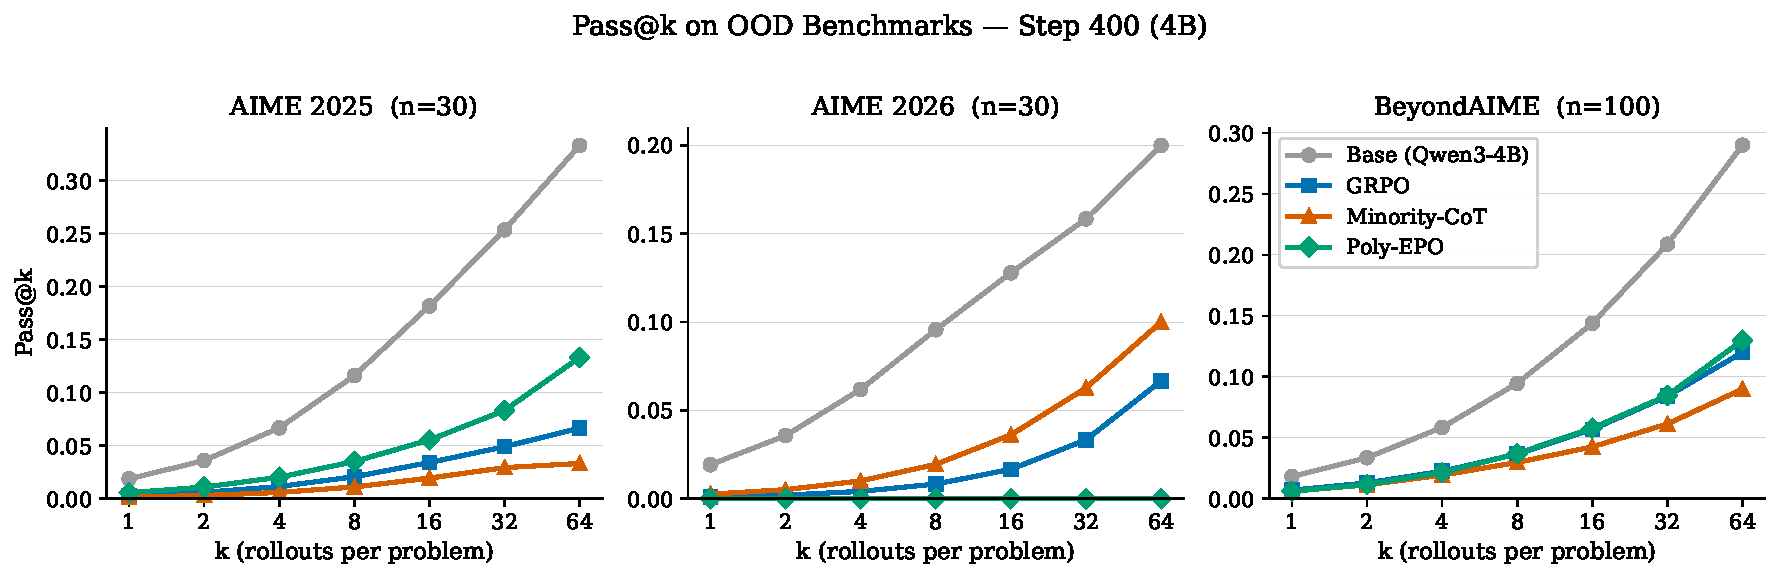
\includegraphics[width=\linewidth]{fig1_passk.pdf}
\caption{Pass@$k$ curves across six benchmarks (2$\times$3 grid, ordered
roughly by difficulty left-to-right, top-to-bottom). The base model (gray)
leads on every benchmark. Trained arms are competitive on in-distribution
MATH-500 and HMMT Nov 2025, but regress substantially on harder OOD benchmarks.
Curves remain roughly parallel on the log-scale $x$-axis, indicating the gap
does not close with more samples.}
\label{fig:passk}
\end{figure}

Figure~\ref{fig:passk} shows pass@$k$ across MATH-500 (in-distribution),
HMMT November 2025, HMMT February 2025, BeyondAIME, AIME 2025, and AIME 2026.
On in-distribution MATH-500, trained arms are competitive with base (pass@16:
base 0.864 vs.\ GRPO 0.711, Poly-EPO 0.707, Minority-CoT 0.683). On HMMT
November 2025, the gap is also small. On harder OOD benchmarks, however, the
base model leads substantially: on BeyondAIME at pass@16, base (0.144)
outperforms the best trained arm by $\approx 2.5\times$.

The gap does not close as $k$ increases --- pass@$k$ curves remain roughly
parallel on the log scale from $k{=}1$ to $k{=}64$ --- indicating that trained
models are not exploring solution strategies the base model finds with more
samples. This is consistent with RL training narrowing the effective support of
the model's solution distribution. Among trained arms, GRPO and Poly-EPO
perform comparably on most benchmarks, with Minority-CoT slightly behind. The
set-RL arms do not improve over GRPO despite being designed to find rare correct
solutions.

% ─────────────────────────────────────────────────────────────────────────────
\subsection{CoT Diversity}
\label{sec:results:cot}
% ─────────────────────────────────────────────────────────────────────────────

Pass@$k$ cannot measure solution diversity on single-answer benchmarks: if a
model gets a problem right, all correct rollouts give the same answer. To test
whether the set-RL arms generate genuinely diverse \emph{reasoning strategies},
we use an LLM judge (Qwen3-4B-Instruct) to cluster rollouts by macro- and
micro-strategy~\citep{polyepo}, then report the average number of distinct
correct CoT clusters per problem, averaged only over problems the model solved
at least once (using all 64 rollouts).

\begin{table}[h]
\centering
\caption{Distinct correct CoT clusters per solved problem. Averaged only over
problems with at least one correct rollout, using all 64 rollouts. Best per
dataset in \textbf{bold}.}
\label{tab:cot}
\small
\setlength{\tabcolsep}{8pt}
\begin{tabular}{llcc}
\toprule
\textbf{Dataset} & \textbf{Arm} & \textbf{\#solved / total} & \textbf{distinct correct CoT clusters} \\
\midrule
\multirow{4}{*}{MATH-500}
  & Base (Qwen3-4B) & \textbf{464} / 500 & \textbf{1.179} \\
  & GRPO            & 408 / 500 & 1.152 \\
  & Poly-EPO        & 405 / 500 & 1.034 \\
  & Minority-CoT    & 402 / 500 & 0.990 \\
\midrule
\multirow{4}{*}{BeyondAIME}
  & Base (Qwen3-4B) & \textbf{29} / 100 & 0.586 \\
  & GRPO            & 12 / 100 & \textbf{0.667} \\
  & Minority-CoT    & 9 / 100  & 0.333 \\
  & Poly-EPO        & 13 / 100 & 0.231 \\
\bottomrule
\end{tabular}
\end{table}

\begin{figure}[h]
\centering
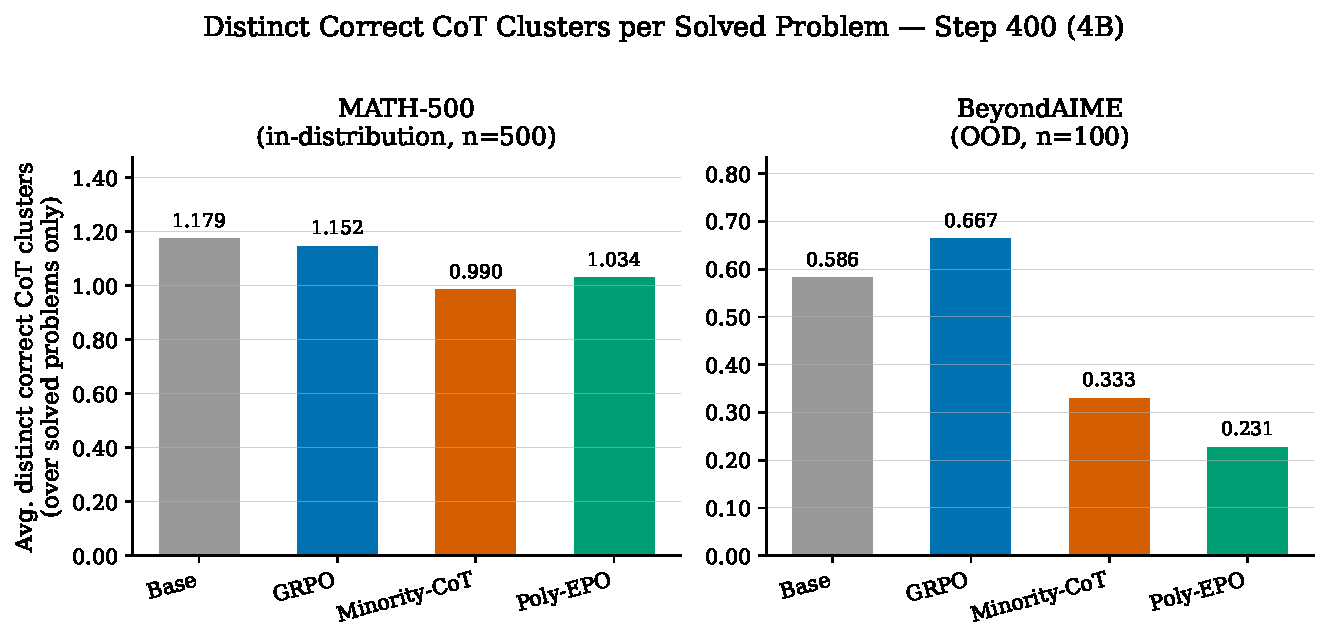
\includegraphics[width=0.9\linewidth]{fig2_cot_diversity.pdf}
\caption{Distinct correct CoT clusters per solved problem on MATH-500
(in-distribution, left) and BeyondAIME (OOD, right). On MATH-500 the base
model leads narrowly. On BeyondAIME, GRPO leads despite solving fewer
problems overall; the set-RL arms (Minority-CoT, Poly-EPO) are lowest on
both benchmarks.}
\label{fig:cot}
\end{figure}

Table~\ref{tab:cot} and Figure~\ref{fig:cot} reveal two distinct patterns. On
MATH-500, the base model (1.179) leads narrowly over GRPO (1.152), with the
set-RL arms below (Poly-EPO 1.034, Minority-CoT 0.990). All four arms generate
roughly one distinct correct reasoning approach per solved problem, consistent
with most MATH-500 problems having a single canonical solution method.

On BeyondAIME, conditioning on solved problems reverses the ordering: GRPO
(0.667) \emph{exceeds} the base model (0.586), while the set-RL arms fall well
below both (Minority-CoT 0.333, Poly-EPO 0.231). The set-RL arms rank last on
the metric they were explicitly trained to maximize. This finding extends to the
correctness axis: the OOD regression from pass@$k$ (Figure~\ref{fig:passk}) is
primarily a loss of \textbf{breadth} (fewer problems solved) rather than
\textbf{depth} (less diverse reasoning per solved problem) --- GRPO's per-problem
diversity actually exceeds base on OOD data.

A confound worth ruling out: the set-RL arms solve slightly fewer problems, which
could reduce opportunities to observe multiple CoT clusters. However, on MATH-500
all four arms solve 402--464 / 500 problems (a narrow 13\% range) yet span 0.19
units in per-problem diversity (0.990--1.179). The diversity reduction in the
set-RL arms reflects a genuine change in the solution-strategy distribution, not
an artifact of lower solve rates.

% ─────────────────────────────────────────────────────────────────────────────
\subsection{Why Set-RL Objectives Underperform GRPO}
\label{sec:results:discussion}
% ─────────────────────────────────────────────────────────────────────────────

The central hypothesis behind Minority-CoT and Poly-EPO is that rewarding
diverse correct solutions within each training batch should produce models that
explore more reasoning strategies at inference time. Our results do not support
this hypothesis. On BeyondAIME, the gap is striking: GRPO (0.667) is $2\times$
Minority-CoT (0.333) and $3\times$ Poly-EPO (0.231) in per-problem CoT
diversity.

One likely mechanism is a \textbf{mode-collapsing effect} of the minority
voting objective. Minority-CoT rewards rollouts that reach the correct answer
via the \emph{least common} reasoning cluster in each batch. If the model learns
to reliably produce this minority-mode answer, it converges toward a narrow
distribution concentrated on that approach, suppressing other valid strategies.
The objective replaces one mode (the common answer) with another (the minority
answer) rather than broadening the distribution.

A second possibility is that the diversity reward is satisfied during training
by \emph{surface variation} (different notation, intermediate steps) rather than
genuinely distinct macro-strategies. If the LLM judge correctly clusters such
variants together at evaluation time, the training-time diversity does not
appear in our metric.

These results suggest two directions for future work:

\begin{enumerate}[leftmargin=*, label=\arabic*.]

\item \textbf{Training distribution.}
Polaris problems may not provide sufficient natural solution diversity for a
useful minority signal. Problems with multiple structurally distinct solution
approaches (e.g., combinatorics problems solvable by direct counting, generating
functions, or recursion) could yield richer cluster structure during training.

\item \textbf{Objective formulation.}
Strengthening the judge prompt to penalize superficially different but
strategically identical rollouts, or adding an answer-level diversity
constraint, could better align the training signal with the desired
generalization behavior.

\end{enumerate}

More broadly, our findings contribute to growing evidence that RL training for
math reasoning trades generalization breadth for in-distribution reliability.
Whether this tradeoff is fundamental or addressable through better training data
and objectives remains an open question.

\end{document}
 from a parent document (remove \documentclass block).

\documentclass[11pt]{article}
\usepackage[margin=1in]{geometry}
\usepackage{booktabs}
\usepackage{graphicx}
\usepackage{amsmath}
\usepackage{amssymb}
\usepackage{hyperref}
\usepackage{xcolor}
\usepackage{microtype}
\usepackage{caption}
\usepackage{subcaption}
\usepackage{multirow}
\usepackage{array}
\usepackage{enumitem}

\hypersetup{colorlinks=true, linkcolor=blue, citecolor=blue, urlcolor=blue}
\captionsetup{font=small, labelfont=bf}

\graphicspath{{./}}   % figures live in the same directory as this .tex file

\begin{document}

% ─────────────────────────────────────────────────────────────────────────────
\section{Results and Discussion}
\label{sec:results}
% ─────────────────────────────────────────────────────────────────────────────

We evaluate all three trained arms (GRPO, Minority-CoT, Poly-EPO) against an
untrained base model (Qwen3-4B-Base) along two axes: \emph{answer coverage}
(pass@$k$) and \emph{reasoning diversity} (distinct correct CoT clusters per
solved problem). All pass@$k$ metrics use the exact unbiased estimator averaged
over all $\binom{n}{k}$ subsets of $k$ rollouts from $n = 64$ total per prompt.

% ─────────────────────────────────────────────────────────────────────────────
\subsection{Pass@\texorpdfstring{$k$}{k}}
\label{sec:results:passk}
% ─────────────────────────────────────────────────────────────────────────────

\begin{figure}[h]
\centering
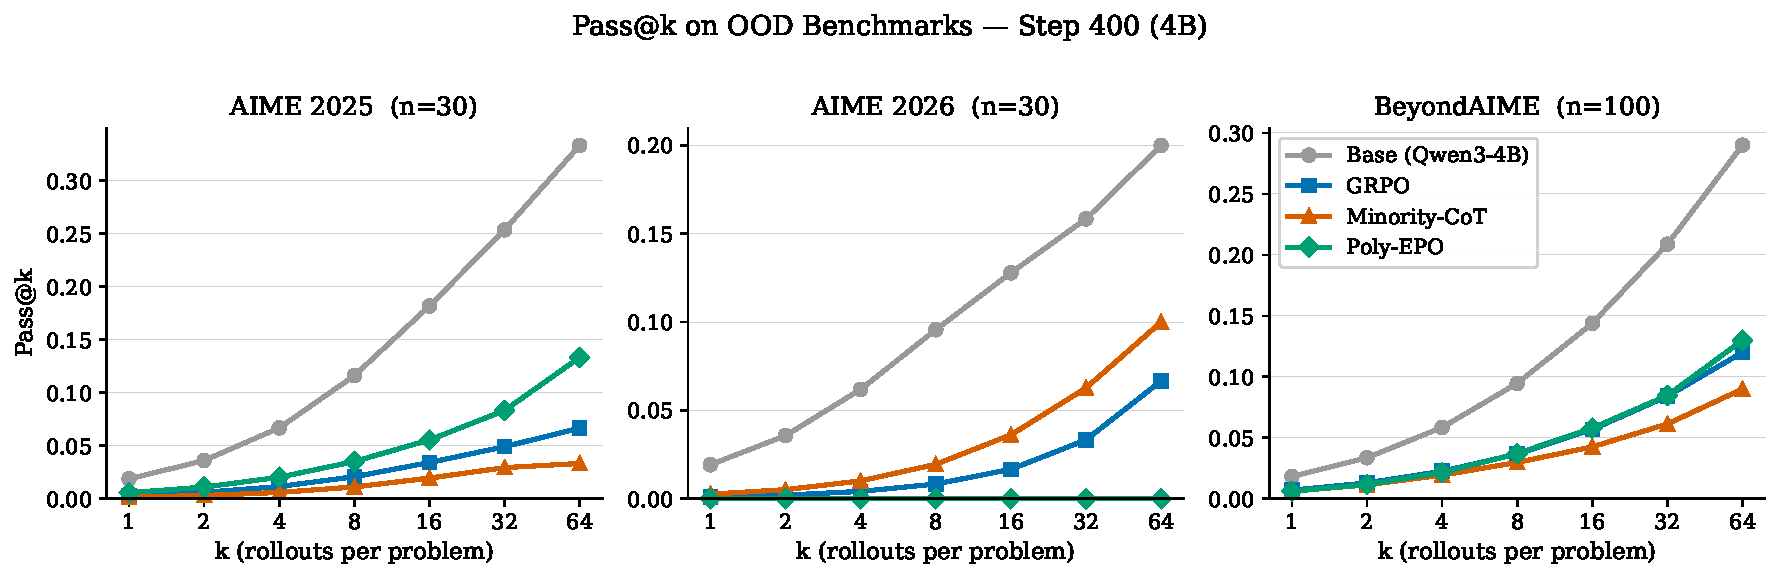
\includegraphics[width=\linewidth]{fig1_passk.pdf}
\caption{Pass@$k$ curves across six benchmarks (2$\times$3 grid, ordered
roughly by difficulty left-to-right, top-to-bottom). The base model (gray)
leads on every benchmark. Trained arms are competitive on in-distribution
MATH-500 and HMMT Nov 2025, but regress substantially on harder OOD benchmarks.
Curves remain roughly parallel on the log-scale $x$-axis, indicating the gap
does not close with more samples.}
\label{fig:passk}
\end{figure}

Figure~\ref{fig:passk} shows pass@$k$ across MATH-500 (in-distribution),
HMMT November 2025, HMMT February 2025, BeyondAIME, AIME 2025, and AIME 2026.
On in-distribution MATH-500, trained arms are competitive with base (pass@16:
base 0.864 vs.\ GRPO 0.711, Poly-EPO 0.707, Minority-CoT 0.683). On HMMT
November 2025, the gap is also small. On harder OOD benchmarks, however, the
base model leads substantially: on BeyondAIME at pass@16, base (0.144)
outperforms the best trained arm by $\approx 2.5\times$.

The gap does not close as $k$ increases --- pass@$k$ curves remain roughly
parallel on the log scale from $k{=}1$ to $k{=}64$ --- indicating that trained
models are not exploring solution strategies the base model finds with more
samples. This is consistent with RL training narrowing the effective support of
the model's solution distribution. Among trained arms, GRPO and Poly-EPO
perform comparably on most benchmarks, with Minority-CoT slightly behind. The
set-RL arms do not improve over GRPO despite being designed to find rare correct
solutions.

% ─────────────────────────────────────────────────────────────────────────────
\subsection{CoT Diversity}
\label{sec:results:cot}
% ─────────────────────────────────────────────────────────────────────────────

Pass@$k$ cannot measure solution diversity on single-answer benchmarks: if a
model gets a problem right, all correct rollouts give the same answer. To test
whether the set-RL arms generate genuinely diverse \emph{reasoning strategies},
we use an LLM judge (Qwen3-4B-Instruct) to cluster rollouts by macro- and
micro-strategy~\citep{polyepo}, then report the average number of distinct
correct CoT clusters per problem, averaged only over problems the model solved
at least once (using all 64 rollouts).

\begin{table}[h]
\centering
\caption{Distinct correct CoT clusters per solved problem. Averaged only over
problems with at least one correct rollout, using all 64 rollouts. Best per
dataset in \textbf{bold}.}
\label{tab:cot}
\small
\setlength{\tabcolsep}{8pt}
\begin{tabular}{llcc}
\toprule
\textbf{Dataset} & \textbf{Arm} & \textbf{\#solved / total} & \textbf{distinct correct CoT clusters} \\
\midrule
\multirow{4}{*}{MATH-500}
  & Base (Qwen3-4B) & \textbf{464} / 500 & \textbf{1.179} \\
  & GRPO            & 408 / 500 & 1.152 \\
  & Poly-EPO        & 405 / 500 & 1.034 \\
  & Minority-CoT    & 402 / 500 & 0.990 \\
\midrule
\multirow{4}{*}{BeyondAIME}
  & Base (Qwen3-4B) & \textbf{29} / 100 & 0.586 \\
  & GRPO            & 12 / 100 & \textbf{0.667} \\
  & Minority-CoT    & 9 / 100  & 0.333 \\
  & Poly-EPO        & 13 / 100 & 0.231 \\
\bottomrule
\end{tabular}
\end{table}

\begin{figure}[h]
\centering
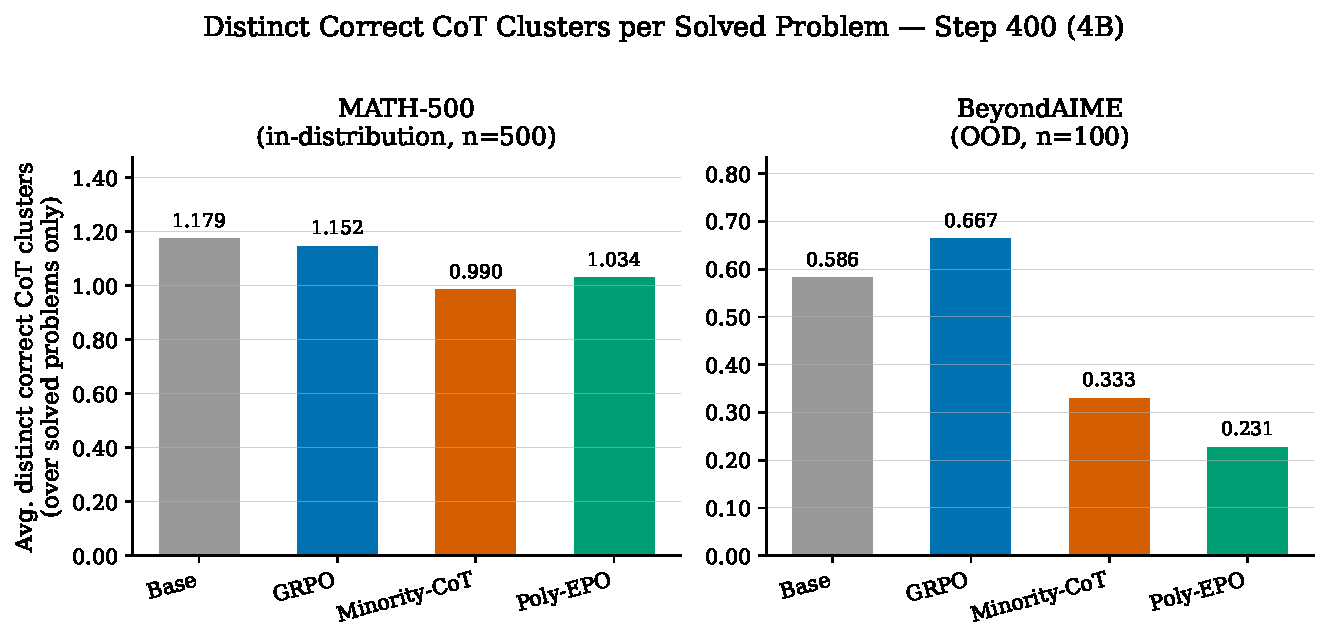
\includegraphics[width=0.9\linewidth]{fig2_cot_diversity.pdf}
\caption{Distinct correct CoT clusters per solved problem on MATH-500
(in-distribution, left) and BeyondAIME (OOD, right). On MATH-500 the base
model leads narrowly. On BeyondAIME, GRPO leads despite solving fewer
problems overall; the set-RL arms (Minority-CoT, Poly-EPO) are lowest on
both benchmarks.}
\label{fig:cot}
\end{figure}

Table~\ref{tab:cot} and Figure~\ref{fig:cot} reveal two distinct patterns. On
MATH-500, the base model (1.179) leads narrowly over GRPO (1.152), with the
set-RL arms below (Poly-EPO 1.034, Minority-CoT 0.990). All four arms generate
roughly one distinct correct reasoning approach per solved problem, consistent
with most MATH-500 problems having a single canonical solution method.

On BeyondAIME, conditioning on solved problems reverses the ordering: GRPO
(0.667) \emph{exceeds} the base model (0.586), while the set-RL arms fall well
below both (Minority-CoT 0.333, Poly-EPO 0.231). The set-RL arms rank last on
the metric they were explicitly trained to maximize. This finding extends to the
correctness axis: the OOD regression from pass@$k$ (Figure~\ref{fig:passk}) is
primarily a loss of \textbf{breadth} (fewer problems solved) rather than
\textbf{depth} (less diverse reasoning per solved problem) --- GRPO's per-problem
diversity actually exceeds base on OOD data.

A confound worth ruling out: the set-RL arms solve slightly fewer problems, which
could reduce opportunities to observe multiple CoT clusters. However, on MATH-500
all four arms solve 402--464 / 500 problems (a narrow 13\% range) yet span 0.19
units in per-problem diversity (0.990--1.179). The diversity reduction in the
set-RL arms reflects a genuine change in the solution-strategy distribution, not
an artifact of lower solve rates.

% ─────────────────────────────────────────────────────────────────────────────
\subsection{Why Set-RL Objectives Underperform GRPO}
\label{sec:results:discussion}
% ─────────────────────────────────────────────────────────────────────────────

The central hypothesis behind Minority-CoT and Poly-EPO is that rewarding
diverse correct solutions within each training batch should produce models that
explore more reasoning strategies at inference time. Our results do not support
this hypothesis. On BeyondAIME, the gap is striking: GRPO (0.667) is $2\times$
Minority-CoT (0.333) and $3\times$ Poly-EPO (0.231) in per-problem CoT
diversity.

One likely mechanism is a \textbf{mode-collapsing effect} of the minority
voting objective. Minority-CoT rewards rollouts that reach the correct answer
via the \emph{least common} reasoning cluster in each batch. If the model learns
to reliably produce this minority-mode answer, it converges toward a narrow
distribution concentrated on that approach, suppressing other valid strategies.
The objective replaces one mode (the common answer) with another (the minority
answer) rather than broadening the distribution.

A second possibility is that the diversity reward is satisfied during training
by \emph{surface variation} (different notation, intermediate steps) rather than
genuinely distinct macro-strategies. If the LLM judge correctly clusters such
variants together at evaluation time, the training-time diversity does not
appear in our metric.

These results suggest two directions for future work:

\begin{enumerate}[leftmargin=*, label=\arabic*.]

\item \textbf{Training distribution.}
Polaris problems may not provide sufficient natural solution diversity for a
useful minority signal. Problems with multiple structurally distinct solution
approaches (e.g., combinatorics problems solvable by direct counting, generating
functions, or recursion) could yield richer cluster structure during training.

\item \textbf{Objective formulation.}
Strengthening the judge prompt to penalize superficially different but
strategically identical rollouts, or adding an answer-level diversity
constraint, could better align the training signal with the desired
generalization behavior.

\end{enumerate}

More broadly, our findings contribute to growing evidence that RL training for
math reasoning trades generalization breadth for in-distribution reliability.
Whether this tradeoff is fundamental or addressable through better training data
and objectives remains an open question.

\end{document}
 from a parent document (remove \documentclass block).

\documentclass[11pt]{article}
\usepackage[margin=1in]{geometry}
\usepackage{booktabs}
\usepackage{graphicx}
\usepackage{amsmath}
\usepackage{amssymb}
\usepackage{hyperref}
\usepackage{xcolor}
\usepackage{microtype}
\usepackage{caption}
\usepackage{subcaption}
\usepackage{multirow}
\usepackage{array}
\usepackage{enumitem}

\hypersetup{colorlinks=true, linkcolor=blue, citecolor=blue, urlcolor=blue}
\captionsetup{font=small, labelfont=bf}

\graphicspath{{./}}   % figures live in the same directory as this .tex file

\begin{document}

% ─────────────────────────────────────────────────────────────────────────────
\section{Results and Discussion}
\label{sec:results}
% ─────────────────────────────────────────────────────────────────────────────

We evaluate all three trained arms (GRPO, Minority-CoT, Poly-EPO) against an
untrained base model (Qwen3-4B-Base) along two axes: \emph{answer coverage}
(pass@$k$) and \emph{reasoning diversity} (distinct correct CoT clusters per
solved problem). All pass@$k$ metrics use the exact unbiased estimator averaged
over all $\binom{n}{k}$ subsets of $k$ rollouts from $n = 64$ total per prompt.

% ─────────────────────────────────────────────────────────────────────────────
\subsection{Pass@\texorpdfstring{$k$}{k}}
\label{sec:results:passk}
% ─────────────────────────────────────────────────────────────────────────────

\begin{figure}[h]
\centering
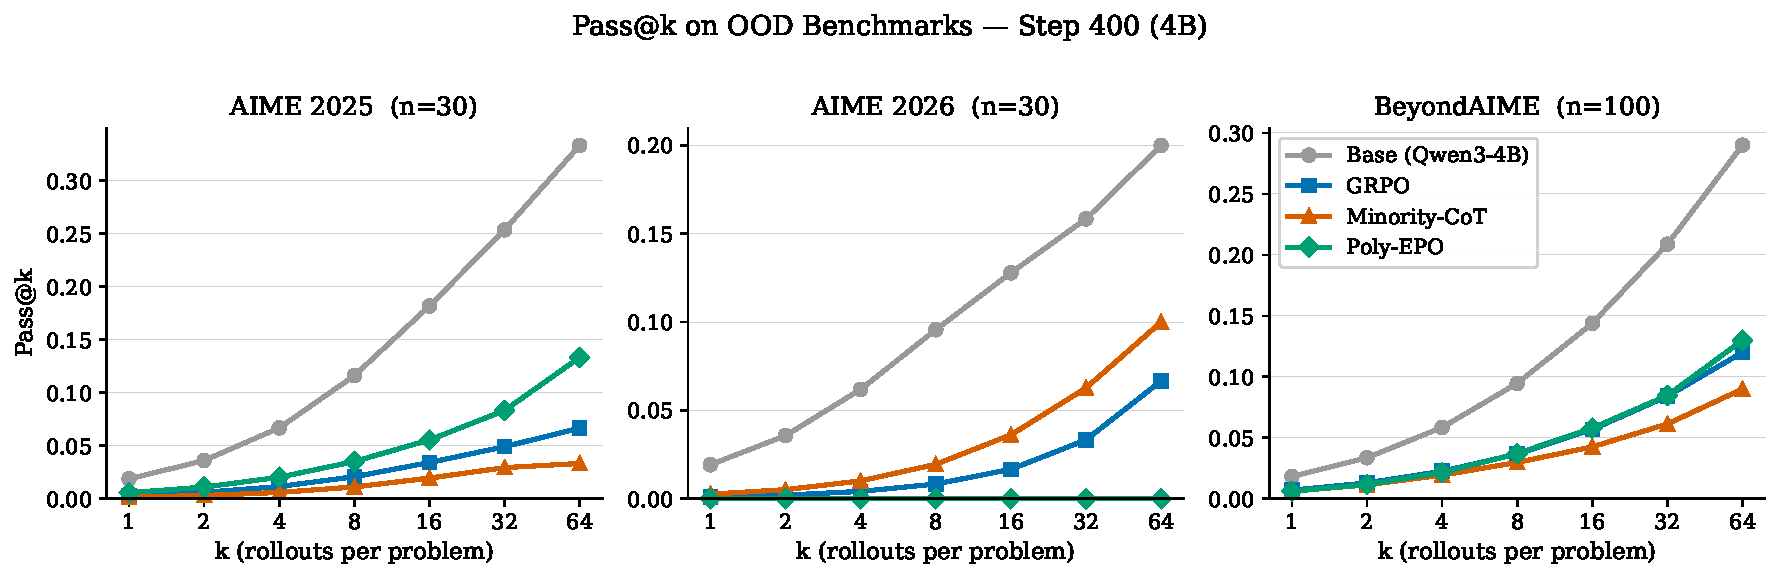
\includegraphics[width=\linewidth]{fig1_passk.pdf}
\caption{Pass@$k$ curves across six benchmarks (2$\times$3 grid, ordered
roughly by difficulty left-to-right, top-to-bottom). The base model (gray)
leads on every benchmark. Trained arms are competitive on in-distribution
MATH-500 and HMMT Nov 2025, but regress substantially on harder OOD benchmarks.
Curves remain roughly parallel on the log-scale $x$-axis, indicating the gap
does not close with more samples.}
\label{fig:passk}
\end{figure}

Figure~\ref{fig:passk} shows pass@$k$ across MATH-500 (in-distribution),
HMMT November 2025, HMMT February 2025, BeyondAIME, AIME 2025, and AIME 2026.
On in-distribution MATH-500, trained arms are competitive with base (pass@16:
base 0.864 vs.\ GRPO 0.711, Poly-EPO 0.707, Minority-CoT 0.683). On HMMT
November 2025, the gap is also small. On harder OOD benchmarks, however, the
base model leads substantially: on BeyondAIME at pass@16, base (0.144)
outperforms the best trained arm by $\approx 2.5\times$.

The gap does not close as $k$ increases --- pass@$k$ curves remain roughly
parallel on the log scale from $k{=}1$ to $k{=}64$ --- indicating that trained
models are not exploring solution strategies the base model finds with more
samples. This is consistent with RL training narrowing the effective support of
the model's solution distribution. Among trained arms, GRPO and Poly-EPO
perform comparably on most benchmarks, with Minority-CoT slightly behind. The
set-RL arms do not improve over GRPO despite being designed to find rare correct
solutions.

% ─────────────────────────────────────────────────────────────────────────────
\subsection{CoT Diversity}
\label{sec:results:cot}
% ─────────────────────────────────────────────────────────────────────────────

Pass@$k$ cannot measure solution diversity on single-answer benchmarks: if a
model gets a problem right, all correct rollouts give the same answer. To test
whether the set-RL arms generate genuinely diverse \emph{reasoning strategies},
we use an LLM judge (Qwen3-4B-Instruct) to cluster rollouts by macro- and
micro-strategy~\citep{polyepo}, then report the average number of distinct
correct CoT clusters per problem, averaged only over problems the model solved
at least once (using all 64 rollouts).

\begin{table}[h]
\centering
\caption{Distinct correct CoT clusters per solved problem. Averaged only over
problems with at least one correct rollout, using all 64 rollouts. Best per
dataset in \textbf{bold}.}
\label{tab:cot}
\small
\setlength{\tabcolsep}{8pt}
\begin{tabular}{llcc}
\toprule
\textbf{Dataset} & \textbf{Arm} & \textbf{\#solved / total} & \textbf{distinct correct CoT clusters} \\
\midrule
\multirow{4}{*}{MATH-500}
  & Base (Qwen3-4B) & \textbf{464} / 500 & \textbf{1.179} \\
  & GRPO            & 408 / 500 & 1.152 \\
  & Poly-EPO        & 405 / 500 & 1.034 \\
  & Minority-CoT    & 402 / 500 & 0.990 \\
\midrule
\multirow{4}{*}{BeyondAIME}
  & Base (Qwen3-4B) & \textbf{29} / 100 & 0.586 \\
  & GRPO            & 12 / 100 & \textbf{0.667} \\
  & Minority-CoT    & 9 / 100  & 0.333 \\
  & Poly-EPO        & 13 / 100 & 0.231 \\
\bottomrule
\end{tabular}
\end{table}

\begin{figure}[h]
\centering
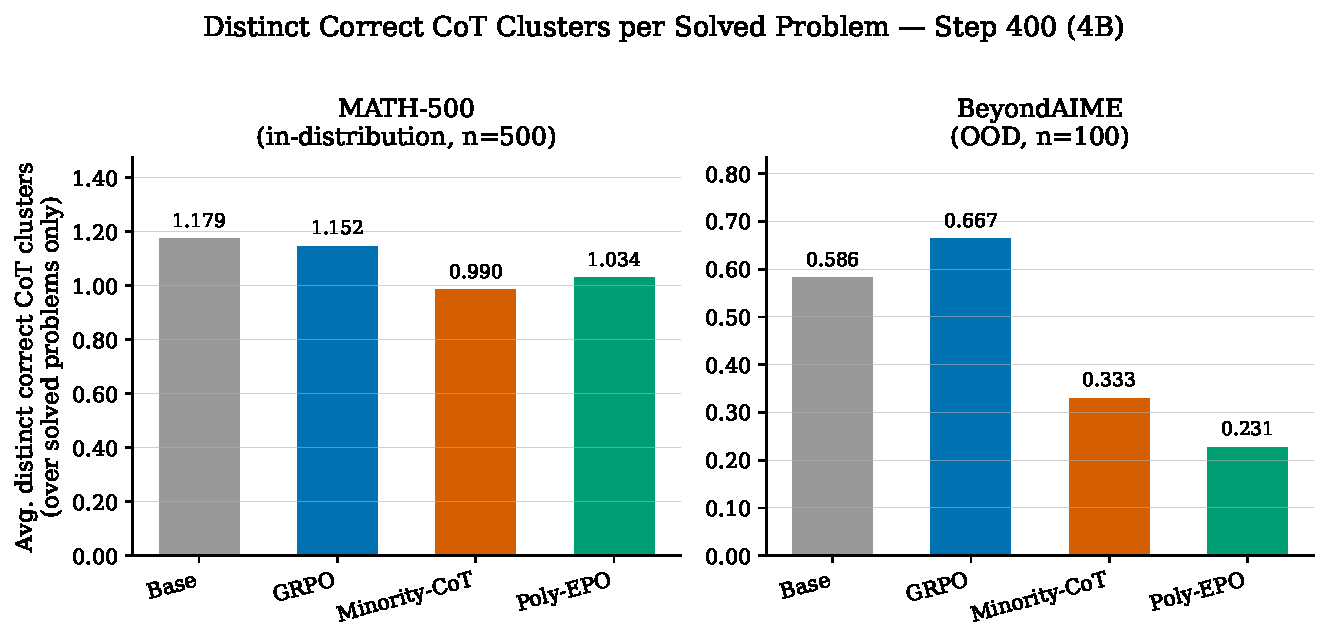
\includegraphics[width=0.9\linewidth]{fig2_cot_diversity.pdf}
\caption{Distinct correct CoT clusters per solved problem on MATH-500
(in-distribution, left) and BeyondAIME (OOD, right). On MATH-500 the base
model leads narrowly. On BeyondAIME, GRPO leads despite solving fewer
problems overall; the set-RL arms (Minority-CoT, Poly-EPO) are lowest on
both benchmarks.}
\label{fig:cot}
\end{figure}

Table~\ref{tab:cot} and Figure~\ref{fig:cot} reveal two distinct patterns. On
MATH-500, the base model (1.179) leads narrowly over GRPO (1.152), with the
set-RL arms below (Poly-EPO 1.034, Minority-CoT 0.990). All four arms generate
roughly one distinct correct reasoning approach per solved problem, consistent
with most MATH-500 problems having a single canonical solution method.

On BeyondAIME, conditioning on solved problems reverses the ordering: GRPO
(0.667) \emph{exceeds} the base model (0.586), while the set-RL arms fall well
below both (Minority-CoT 0.333, Poly-EPO 0.231). The set-RL arms rank last on
the metric they were explicitly trained to maximize. This finding extends to the
correctness axis: the OOD regression from pass@$k$ (Figure~\ref{fig:passk}) is
primarily a loss of \textbf{breadth} (fewer problems solved) rather than
\textbf{depth} (less diverse reasoning per solved problem) --- GRPO's per-problem
diversity actually exceeds base on OOD data.

A confound worth ruling out: the set-RL arms solve slightly fewer problems, which
could reduce opportunities to observe multiple CoT clusters. However, on MATH-500
all four arms solve 402--464 / 500 problems (a narrow 13\% range) yet span 0.19
units in per-problem diversity (0.990--1.179). The diversity reduction in the
set-RL arms reflects a genuine change in the solution-strategy distribution, not
an artifact of lower solve rates.

% ─────────────────────────────────────────────────────────────────────────────
\subsection{Why Set-RL Objectives Underperform GRPO}
\label{sec:results:discussion}
% ─────────────────────────────────────────────────────────────────────────────

The central hypothesis behind Minority-CoT and Poly-EPO is that rewarding
diverse correct solutions within each training batch should produce models that
explore more reasoning strategies at inference time. Our results do not support
this hypothesis. On BeyondAIME, the gap is striking: GRPO (0.667) is $2\times$
Minority-CoT (0.333) and $3\times$ Poly-EPO (0.231) in per-problem CoT
diversity.

One likely mechanism is a \textbf{mode-collapsing effect} of the minority
voting objective. Minority-CoT rewards rollouts that reach the correct answer
via the \emph{least common} reasoning cluster in each batch. If the model learns
to reliably produce this minority-mode answer, it converges toward a narrow
distribution concentrated on that approach, suppressing other valid strategies.
The objective replaces one mode (the common answer) with another (the minority
answer) rather than broadening the distribution.

A second possibility is that the diversity reward is satisfied during training
by \emph{surface variation} (different notation, intermediate steps) rather than
genuinely distinct macro-strategies. If the LLM judge correctly clusters such
variants together at evaluation time, the training-time diversity does not
appear in our metric.

These results suggest two directions for future work:

\begin{enumerate}[leftmargin=*, label=\arabic*.]

\item \textbf{Training distribution.}
Polaris problems may not provide sufficient natural solution diversity for a
useful minority signal. Problems with multiple structurally distinct solution
approaches (e.g., combinatorics problems solvable by direct counting, generating
functions, or recursion) could yield richer cluster structure during training.

\item \textbf{Objective formulation.}
Strengthening the judge prompt to penalize superficially different but
strategically identical rollouts, or adding an answer-level diversity
constraint, could better align the training signal with the desired
generalization behavior.

\end{enumerate}

More broadly, our findings contribute to growing evidence that RL training for
math reasoning trades generalization breadth for in-distribution reliability.
Whether this tradeoff is fundamental or addressable through better training data
and objectives remains an open question.

\end{document}
 from a parent document (remove \documentclass block).

\documentclass[11pt]{article}
\usepackage[margin=1in]{geometry}
\usepackage{booktabs}
\usepackage{graphicx}
\usepackage{amsmath}
\usepackage{amssymb}
\usepackage{hyperref}
\usepackage{xcolor}
\usepackage{microtype}
\usepackage{caption}
\usepackage{subcaption}
\usepackage{multirow}
\usepackage{array}
\usepackage{enumitem}

\hypersetup{colorlinks=true, linkcolor=blue, citecolor=blue, urlcolor=blue}
\captionsetup{font=small, labelfont=bf}

\graphicspath{{./}}   % figures live in the same directory as this .tex file

\begin{document}

% ─────────────────────────────────────────────────────────────────────────────
\section{Results and Discussion}
\label{sec:results}
% ─────────────────────────────────────────────────────────────────────────────

We evaluate all three trained arms (GRPO, Minority-CoT, Poly-EPO) against an
untrained base model (Qwen3-4B-Base) along two axes: \emph{answer coverage}
(pass@$k$) and \emph{reasoning diversity} (distinct correct CoT clusters per
solved problem). All pass@$k$ metrics use the exact unbiased estimator averaged
over all $\binom{n}{k}$ subsets of $k$ rollouts from $n = 64$ total per prompt.

% ─────────────────────────────────────────────────────────────────────────────
\subsection{Pass@\texorpdfstring{$k$}{k}}
\label{sec:results:passk}
% ─────────────────────────────────────────────────────────────────────────────

\begin{figure}[h]
\centering
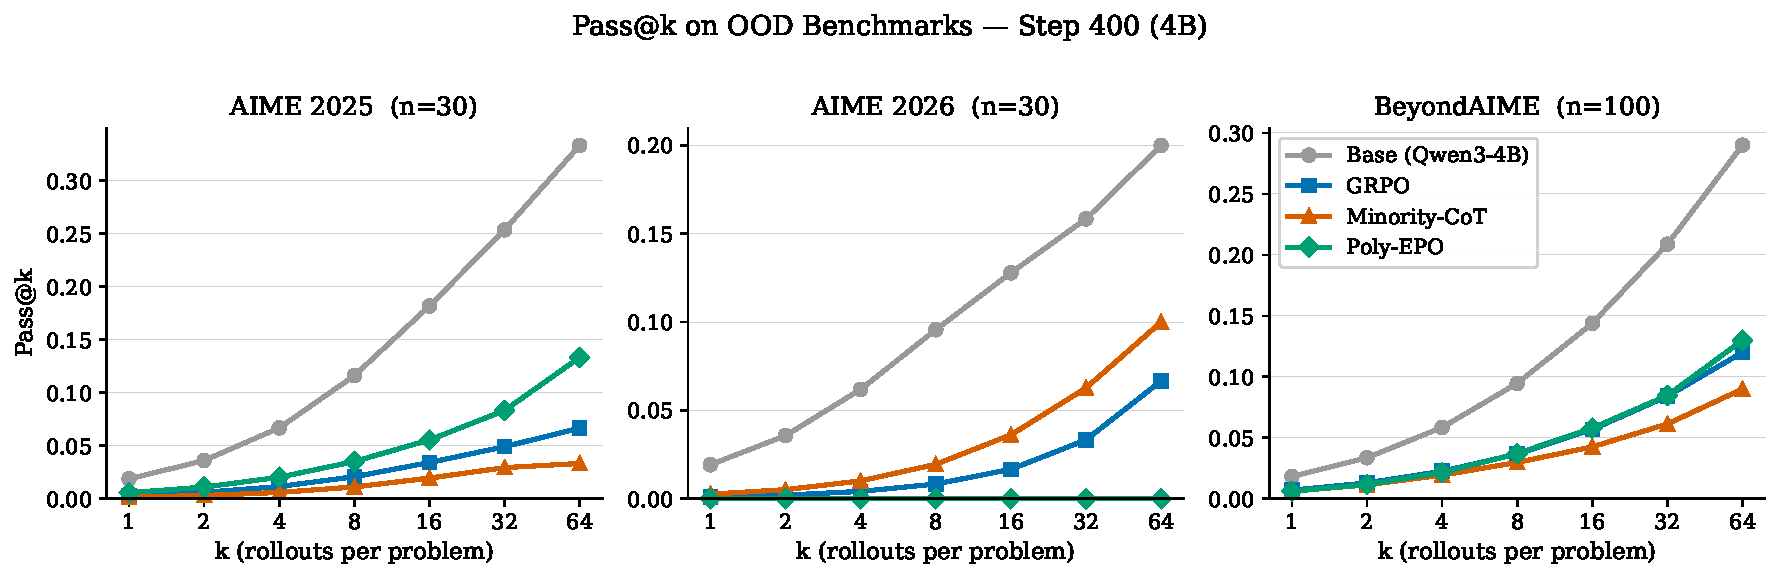
\includegraphics[width=\linewidth]{fig1_passk.pdf}
\caption{Pass@$k$ curves across six benchmarks (2$\times$3 grid, ordered
roughly by difficulty left-to-right, top-to-bottom). The base model (gray)
leads on every benchmark. Trained arms are competitive on in-distribution
MATH-500 and HMMT Nov 2025, but regress substantially on harder OOD benchmarks.
Curves remain roughly parallel on the log-scale $x$-axis, indicating the gap
does not close with more samples.}
\label{fig:passk}
\end{figure}

Figure~\ref{fig:passk} shows pass@$k$ across MATH-500 (in-distribution),
HMMT November 2025, HMMT February 2025, BeyondAIME, AIME 2025, and AIME 2026.
On in-distribution MATH-500, trained arms are competitive with base (pass@16:
base 0.864 vs.\ GRPO 0.711, Poly-EPO 0.707, Minority-CoT 0.683). On HMMT
November 2025, the gap is also small. On harder OOD benchmarks, however, the
base model leads substantially: on BeyondAIME at pass@16, base (0.144)
outperforms the best trained arm by $\approx 2.5\times$.

The gap does not close as $k$ increases --- pass@$k$ curves remain roughly
parallel on the log scale from $k{=}1$ to $k{=}64$ --- indicating that trained
models are not exploring solution strategies the base model finds with more
samples. This is consistent with RL training narrowing the effective support of
the model's solution distribution. Among trained arms, GRPO and Poly-EPO
perform comparably on most benchmarks, with Minority-CoT slightly behind. The
set-RL arms do not improve over GRPO despite being designed to find rare correct
solutions.

% ─────────────────────────────────────────────────────────────────────────────
\subsection{CoT Diversity}
\label{sec:results:cot}
% ─────────────────────────────────────────────────────────────────────────────

Pass@$k$ cannot measure solution diversity on single-answer benchmarks: if a
model gets a problem right, all correct rollouts give the same answer. To test
whether the set-RL arms generate genuinely diverse \emph{reasoning strategies},
we use an LLM judge (Qwen3-4B-Instruct) to cluster rollouts by macro- and
micro-strategy~\citep{polyepo}, then report the average number of distinct
correct CoT clusters per problem, averaged only over problems the model solved
at least once (using all 64 rollouts).

\begin{table}[h]
\centering
\caption{Distinct correct CoT clusters per solved problem. Averaged only over
problems with at least one correct rollout, using all 64 rollouts. Best per
dataset in \textbf{bold}.}
\label{tab:cot}
\small
\setlength{\tabcolsep}{8pt}
\begin{tabular}{llcc}
\toprule
\textbf{Dataset} & \textbf{Arm} & \textbf{\#solved / total} & \textbf{distinct correct CoT clusters} \\
\midrule
\multirow{4}{*}{MATH-500}
  & Base (Qwen3-4B) & \textbf{464} / 500 & \textbf{1.179} \\
  & GRPO            & 408 / 500 & 1.152 \\
  & Poly-EPO        & 405 / 500 & 1.034 \\
  & Minority-CoT    & 402 / 500 & 0.990 \\
\midrule
\multirow{4}{*}{BeyondAIME}
  & Base (Qwen3-4B) & \textbf{29} / 100 & 0.586 \\
  & GRPO            & 12 / 100 & \textbf{0.667} \\
  & Minority-CoT    & 9 / 100  & 0.333 \\
  & Poly-EPO        & 13 / 100 & 0.231 \\
\bottomrule
\end{tabular}
\end{table}

\begin{figure}[h]
\centering
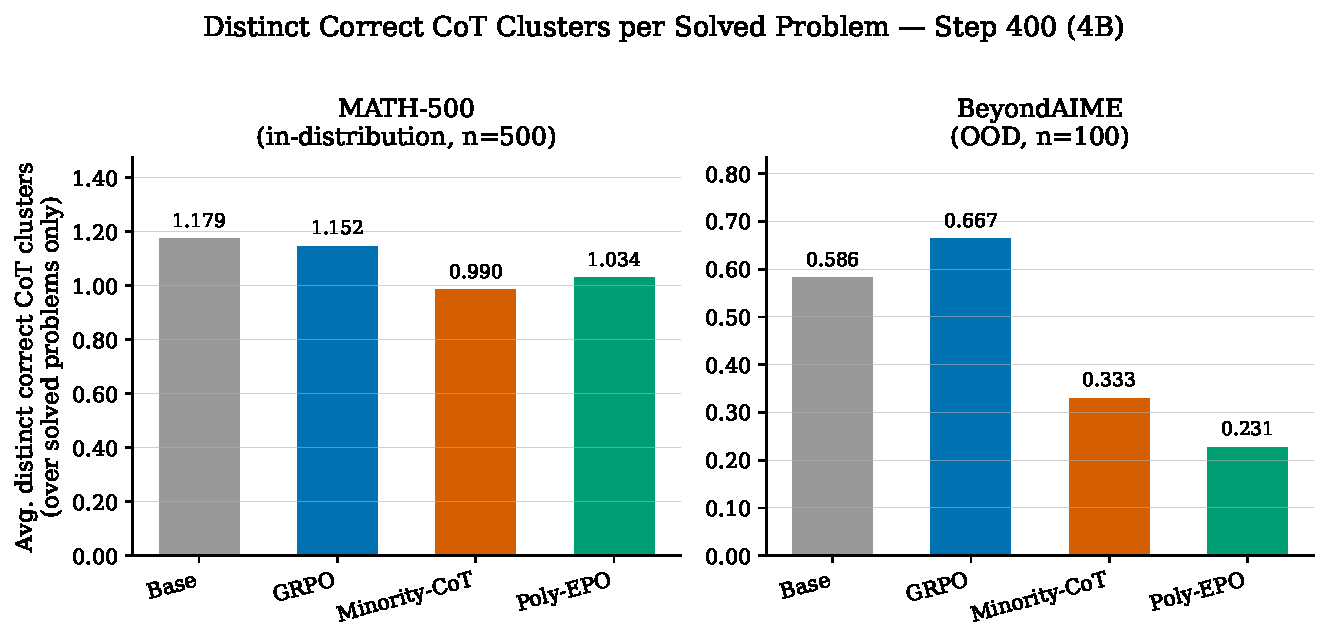
\includegraphics[width=0.9\linewidth]{fig2_cot_diversity.pdf}
\caption{Distinct correct CoT clusters per solved problem on MATH-500
(in-distribution, left) and BeyondAIME (OOD, right). On MATH-500 the base
model leads narrowly. On BeyondAIME, GRPO leads despite solving fewer
problems overall; the set-RL arms (Minority-CoT, Poly-EPO) are lowest on
both benchmarks.}
\label{fig:cot}
\end{figure}

Table~\ref{tab:cot} and Figure~\ref{fig:cot} reveal two distinct patterns. On
MATH-500, the base model (1.179) leads narrowly over GRPO (1.152), with the
set-RL arms below (Poly-EPO 1.034, Minority-CoT 0.990). All four arms generate
roughly one distinct correct reasoning approach per solved problem, consistent
with most MATH-500 problems having a single canonical solution method.

On BeyondAIME, conditioning on solved problems reverses the ordering: GRPO
(0.667) \emph{exceeds} the base model (0.586), while the set-RL arms fall well
below both (Minority-CoT 0.333, Poly-EPO 0.231). The set-RL arms rank last on
the metric they were explicitly trained to maximize. This finding extends to the
correctness axis: the OOD regression from pass@$k$ (Figure~\ref{fig:passk}) is
primarily a loss of \textbf{breadth} (fewer problems solved) rather than
\textbf{depth} (less diverse reasoning per solved problem) --- GRPO's per-problem
diversity actually exceeds base on OOD data.

A confound worth ruling out: the set-RL arms solve slightly fewer problems, which
could reduce opportunities to observe multiple CoT clusters. However, on MATH-500
all four arms solve 402--464 / 500 problems (a narrow 13\% range) yet span 0.19
units in per-problem diversity (0.990--1.179). The diversity reduction in the
set-RL arms reflects a genuine change in the solution-strategy distribution, not
an artifact of lower solve rates.

% ─────────────────────────────────────────────────────────────────────────────
\subsection{Why Set-RL Objectives Underperform GRPO}
\label{sec:results:discussion}
% ─────────────────────────────────────────────────────────────────────────────

The central hypothesis behind Minority-CoT and Poly-EPO is that rewarding
diverse correct solutions within each training batch should produce models that
explore more reasoning strategies at inference time. Our results do not support
this hypothesis. On BeyondAIME, the gap is striking: GRPO (0.667) is $2\times$
Minority-CoT (0.333) and $3\times$ Poly-EPO (0.231) in per-problem CoT
diversity.

One likely mechanism is a \textbf{mode-collapsing effect} of the minority
voting objective. Minority-CoT rewards rollouts that reach the correct answer
via the \emph{least common} reasoning cluster in each batch. If the model learns
to reliably produce this minority-mode answer, it converges toward a narrow
distribution concentrated on that approach, suppressing other valid strategies.
The objective replaces one mode (the common answer) with another (the minority
answer) rather than broadening the distribution.

A second possibility is that the diversity reward is satisfied during training
by \emph{surface variation} (different notation, intermediate steps) rather than
genuinely distinct macro-strategies. If the LLM judge correctly clusters such
variants together at evaluation time, the training-time diversity does not
appear in our metric.

These results suggest two directions for future work:

\begin{enumerate}[leftmargin=*, label=\arabic*.]

\item \textbf{Training distribution.}
Polaris problems may not provide sufficient natural solution diversity for a
useful minority signal. Problems with multiple structurally distinct solution
approaches (e.g., combinatorics problems solvable by direct counting, generating
functions, or recursion) could yield richer cluster structure during training.

\item \textbf{Objective formulation.}
Strengthening the judge prompt to penalize superficially different but
strategically identical rollouts, or adding an answer-level diversity
constraint, could better align the training signal with the desired
generalization behavior.

\end{enumerate}

More broadly, our findings contribute to growing evidence that RL training for
math reasoning trades generalization breadth for in-distribution reliability.
Whether this tradeoff is fundamental or addressable through better training data
and objectives remains an open question.

\end{document}
